\clearpage

\phantomsection\section*{\hypertarget{appendix}{Appendix: RLH simulation code}}
\addcontentsline{toc}{section}{Appendix: RLH simulation code}
\renewcommand\thesubsection{\thesection\Alph{subsection}}

\pagestyle{fancy}
\fancyhf{}
\renewcommand{\headrulewidth}{0pt}
\cfoot{\thepage}
\chead{\nouppercase{\sc Appendix}}

This appendix provides standalone \texttt{python} code (tested with \texttt{v3.7.3}) which demonstrates how the RLH polygons from \autoref{def:rlh_polygon} may be simulated. The code is self explanatory, except:~we denote $\hat W^\alpha$ and $\hat W^\rho$ by \texttt{Wa} and \texttt{Wr}; the \texttt{kernel} array contains the evaluation points $(x^*_k)^{-\alpha}$ from \autoref{eq:RL_polygon}, and; \texttt{np.convolve} evaluates \emph{all} sums in \autoref{eq:RL_polygon} simultaneously, like in \cite{bennedsen_2017}. This code takes $75\pm1$ ms to run on a 2.3 GHz Intel Core i5 MacBook Pro, and the arrays \texttt{V} and \texttt{S} from it are illustrated in \autoref{fig:simulation_output}.

\vspace{2mm}
\begin{figure}[ht]
    \centering
    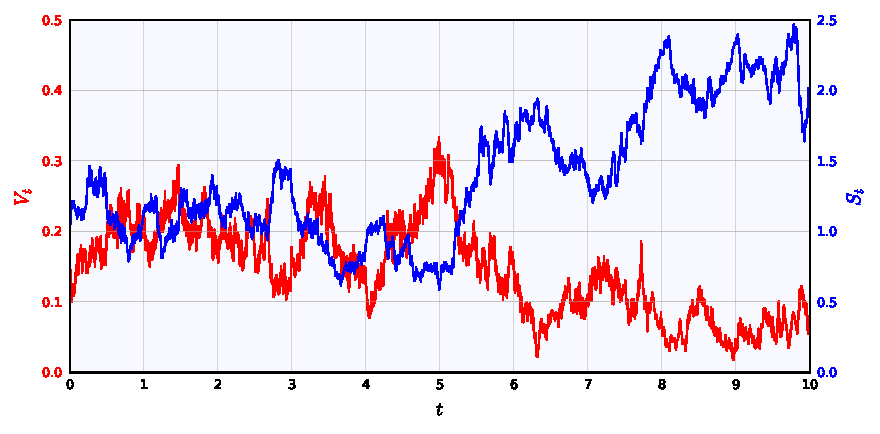
\includegraphics[width=1.0\linewidth]{figures/code_output}
    \caption{The data in the \texttt{V} and \texttt{S} arrays is shown, after running the \texttt{python} code below with the given seed. This may be compared with Figure 1 in \cite{gatheral_2020}.}
    \label{fig:simulation_output}
\end{figure}

\vspace{-2mm}
\begin{linenumbers}
\texttt{import numpy as np\\
from scipy.special import gamma\\
from scipy.interpolate import interp1d\\
{\color{alt3}\emph{\# Set RLH model parameters, which coincide with Heston's for alpha = 0}}\\
sigma, alpha, kappa, theta, v, rho = 0.1, 0.2, 0.3, 0.4**2, 0.4**2, -0.5\\
{\color{alt3}\emph{\# Set simulation horizons and discretisation steps}}\\
time\_horizon, space\_horizon = 10.0, 1.6\\
time\_steps, space\_steps = 4096, 4096\\
{\color{alt3}\emph{\# Build time and space arrays for forward Euler scheme and random field}}\\
dt = time\_horizon / time\_steps\\
t = np.linspace(0, time\_horizon, time\_steps + 1)\\
dx = space\_horizon / space\_steps\\
x = np.linspace(0, space\_horizon, space\_steps + 1)\\
{\color{alt3}\emph{\# Draw Brownian increments and build Brownian motions}}\\
np.random.seed(1)\\
dW = np.random.normal(size=(space\_steps, 2)) * dx**0.5\\
W = np.zeros((space\_steps + 1, 2))\\
W[1:, :]~= np.cumsum(dW, axis=0)\\
Wr = rho * W[:, 1] + (1 - rho**2)**0.5 * W[:, 0]\\
{\color{alt3}\emph{\# Compute the fractional derivative Wa of W1 using \autoref{eq:RL_polygon}}}\\
Wa = np.zeros(space\_steps + 1)\\
kernel = (x[1:]**(1 - alpha) - x[:-1]**(1 - alpha)) / (1 - alpha) / dx\\
Wa[1:]~= np.convolve(kernel, dW[:, 1])[:space\_steps] / gamma(1 - alpha)\\
{\color{alt3}\emph{\# Build linearly interpolating polygons}}\\
Wa\_polygon = interp1d(x, Wa)\\
Wr\_polygon = interp1d(x, Wr)\\
{\color{alt3}\emph{\# Approximate the RLH random field from \autoref{def:gen_hest_field3}}}\\
def Y(t, x):\\
{\color{white}oooo}return sigma * Wa\_polygon(x) + kappa * (theta * t - x) + v\\
{\color{alt3}\emph{\# Conduct basic forward Euler scheme for cumulative variance X}}\\
V = np.zeros(time\_steps)\\
X = np.zeros(time\_steps + 1)\\
for i in range(time\_steps):\\
{\color{white}oooo}V[i] = Y(t[i], X[i])\\
{\color{white}oooo}X[i + 1] = X[i] + V[i] * dt\\
{\color{alt3}\emph{\# Construct price path}}\\
S = np.exp(Wr\_polygon(X) - 0.5 * X)
}
\end{linenumbers}
